\documentclass[a4paper]{article}

%% Language and font encodings
\usepackage[english]{babel}
\usepackage[utf8x]{inputenc}
\usepackage[T1]{fontenc}

%% Sets page size and margins
\usepackage[a4paper,top=3cm,bottom=2cm,left=3cm,right=3cm,marginparwidth=1.75cm]{geometry}

%% Useful packages
\usepackage{amsmath}
\usepackage{graphicx}
\usepackage[colorinlistoftodos]{todonotes}
\usepackage[colorlinks=true, allcolors=blue]{hyperref}

\title{Report: Don't Get Kicked}
\author{Ruimin Wang}
\date{}

\begin{document}
\maketitle

\section{Preface}
Language: Python3.6\\
Dependency: pandas, sklearn, gensim\\
Completion Time: 3hrs\\

In this short report I will talking about how my solution for this project works and why I made some decisions the way I did, and what can be done further.

The code can be found at. prepoc.py is the script that will process the raw datafile and transformed it to a directly usable file to machine models; dev.py is the script for selecting models through the train set; And train\_test.py the the final script that will train the selected model and make predictions to the test set. However, I'm not able to fully present how I explored the dataset and how I selected the model with code, I do left some of those codes commended in the lines but many others are not able to be presented that way.

\section{Data Processing/Feature Engineering}

I'll talk about How I treated each attribute by columns

\begin{itemize}
\item "PurcDate": ignored; since it's not likely to be helpful, and hard to do feature engineering on.
\item "VNZIP": ignored; since it's too sparse and not likely to be important given the existent of column "VNST".
\item "VechYear","wheeltype": ignored; since they are identical to other columns
\item "VehicleAge", "VehOdo", "VehBCost", "WarrantyCost": no processing; Since those data are already ordinal numerics.
\item "***Price": replaced value 0 and 1 to NULL, otherwise intact;
\item "Auction", "Make", "Color", "Transmission", "WheelTypeID", "Nationality", "Size", "TopThreeAmericanName", "PRIMEUNIT", "AUCGUART", "VNST", "IsOnlineSale": treated as categorical data and transformed to one-hot vector. Categories only appears in testset are treated as NULL.
\item "BYRNO": similar to above, but transformed infrequent categories to an "other" category
\item "Model", "Trim", "SubModel": those three columns are first appended together, tokenized by whitespace, and then processing by a BoW model that output a 0-1 BoW matrix. Infrequent tokens are filtered out; The reason behind is that this three columns consists of strings composed by tokens of model names, car types, liter numbers and etc. And, those tokens may appear in any of those three columns among different entries.
\end{itemize}

Missing values are represented as a all 0 vector if the data is categorical, or replaced with median of all other values if it is in those "***price" columns.

\section{Evaluation Metrics}
The official metric of this problem is gini index, which is a linear transformation of AUC score, so I made AUC the target of tuning, and calculated gini as well. This metric do makes the most sense here since FPs and FNs would have very different cost here and manually adjust the decision threshold based on ROC may be desired.

Additionally, precision, recall and f-1 is calculated for the positive class given decision threshold 0.5. Among them, recall is considered more important.

\section{Model selecting}
The train set is used as dev propose by testing models with 5-fold cv on it.

To select a proper model, I tried a few basic models with their default parameters, and compares their AUC score. Then, a concise grid search of parameters is performed on the best model.

Among models tried, LR turns out to be the best, Random Forest can get a rather high precision score but AUC and recall seems more important here. A single Decision Tree is not performing good and kernel SVM is much too slow.

parameter tuning shows that the model performs equally good when the regularization constant C is in range [0.01,100], while training is much faster with smaller C value, 0.01 is chosen.

Additionally, each training instance is assigned a weight inverse proportional to frequency of its class, to address the imbalance of that data.

\section{Training \& Prediction}
The selected model is trained on entire train set then and the train model is used to make predictions on testset.

\section{Result}
Due to that label of testset is not given, the result reported here is the scores of the best model during model selecting.

The confusion matrix is given in table \ref{confusion}, and metrics are shown in \ref{metrics}. We can see that this model got a 63.28\% recall on the "Kicked" class with 27.70\% FPR, which means, given decision threshold to be 50\%, this model can avoid 63.28\% of bad buys with the scarface of missing 27.70\% good buy. Moreover, due to it got a AUC of 0.7345, by adjusting the decision threshold based of cost of FNs and FPs to minimize the total cost, it can yield a rather optimal solution. The ROC curve is given in figure\ref{roc}

To compare this model to those in Kaggle, gini index is computed as $auc*2-1$, which turns out 0.4894. This is much to high compared those of test set on Kaggle, so something must be wrong\footnote{Computing gini using predict output of threshold 0.5 instead of probability estimate yield result of 0.3558, which is still higher than best on Kaggle despite that this result is on train set. And this way do makes less sense.} and/or this model may got a severe overfitting.

\begin{table}[]
\centering
\caption{Confusion Matrix}
\label{confusion}
\begin{tabular}{|l|l|}
\hline
TP:5680 & FP:17731 \\ \hline
FN:3296 & TF:46276 \\ \hline
\end{tabular}
\end{table}

\begin{table}[]
\centering
\caption{Metrics}
\label{metrics}
\begin{tabular}{|l|l|l|l|l|}
\hline
AUC    & Gini   & Precision & Recall & F1     \\ \hline
0.7447 & 0.4894 & 0.2426    & 0.6328 & 0.3508 \\ \hline
\end{tabular}
\end{table}

\begin{figure}
\centering
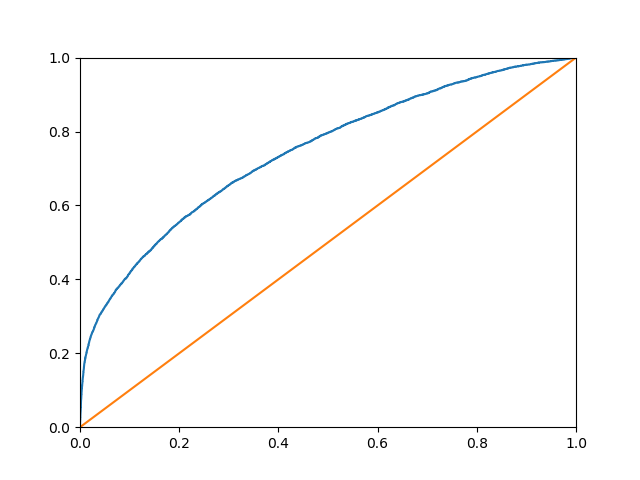
\includegraphics[width=0.5\linewidth]{Figure_1.png}
\caption{ROC curve}
\label{roc}
\end{figure}

\section{Futher works}
\begin{itemize}
\item Some domain knowledge of car dealing industry is desired for further processing of the data. Like, the model/submodel attribute may need some regularization to merge terms of the same meaning. And those domain knowledges may be used to engineering new features out of all those prices
\item The performance of those basic models do indicates this data is hardly separable, and given that LR works out the best, it is worthy to try some simple neuron network model
\item This problem is sensitive to different costs of each instances, not only that Fps and FNs got different cost, but also that each car of different make/cost imply a different cost. But a predictor aware of those factors may be more desirable.
\end{itemize}

\end{document}